
\begin{wrapfigure}{l}{0.25\textwidth}
    \centering
    \caption{Figure 1}
    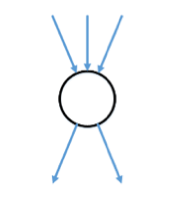
\includegraphics[width=0.25\textwidth]{Fig/figure1.png}
\end{wrapfigure}


%\vspace{1.5cm}


The Codelet model is a fine-grained multi-threaded parallel program execution model based on data flow architecture. Codelet is the finest granularity of parallel units. Each Codelet contains a set of machine instructions, as shown in Figure 1. During the scheduling process, each Codelet is considered as atomic operation. Once the CPU executes a Codelet, it will not be interrupted or migrated to another CPU by the scheduling policy until all the instructions contained in the Codelet are finished, i.e. non-preemptive run. Moreover, since CPU does not have to pay for the overhead of switching between Codelets (saving context, registers, etc.), the Codelet model achieves high efficiency while maintaining fine-grained threading.
%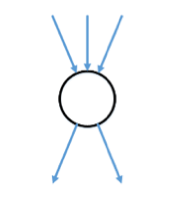
\includegraphics{Fig/figure1.png}

\subsection*{Firing Rules}
When a Codelet receives signals from each of the preceding Codelets (i.e. all dependencies are satisfied), the Codelet will be fired - sent to CPU for execution by scheduling policy. The execution of a Codelet consists of three steps: 1) resetting all predecessors, 2) executing internal machine instructions, 3) generating output results, releasing machine resources and sending signals to subsequent Codelets.
\subsection*{Codelet Graph (CDG)}
Since Codelets are data / event driven, Codelet models do not follow the order of a list of instructions, but instead rely on data / resource dependencies. After the completion of a Codelet, it will produce the corresponding output and release machine resources, while other Codelets may depend on such resources or data. The directional connected graph determined by these dependencies is Codelet Graph (CDG). The nodes in the CDG represent Codelets, the directed edges represent the data dependencies between Codelets, and Figure 2 shows a Codelet Graph.
\subsection*{Threaded Procedure (TP)}
To achieve a higher degree of concurrency, CDG can be partitioned into several subgraphs based on function or execution duration for parallel execution on different CPUs. The Threaded Procedure (TP) is a container for these subgraphs. TP is similar to an asynchronous function and is usually called by other TPs or initialized by the main program. When a TP is called, its corresponding local CDG is also initialized and added to the global CDG. Therefore, the TP provides a way to expand the global CDG. At the same time, TP also plays a role in data locality. When Codelets in a TP share same data or have internal data dependency, these data will be stored in the cache corresponding to the TP to save memory access time. After all the Codelets in the TP are executed, the TP is deleted, and the corresponding local CDG is also removed from the global CDG. Figure 2 shows the mutual relationship between the four TPs.


\begin{figure}[h]
\caption{Figure 2}
\centering
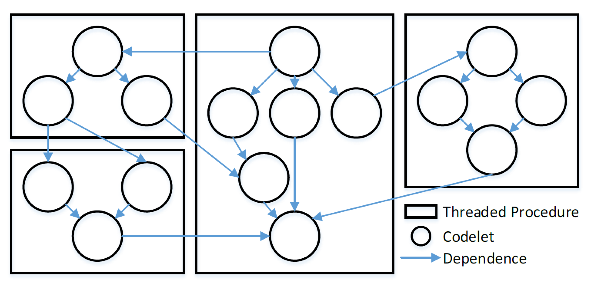
\includegraphics[]{Fig/figure2.png}
\end{figure}
%\textcolor{red}{Figure 2}


\subsection*{Codelet Abstract Machine Model (AMM)} The Codelet Abstract Machine Model describes a hierarchical abstract computer structure that a Codelet model follows during execution, which is not a real computer architecture but rather a map of it. Codelet abstraction machine model consists of many computing nodes, each computing node contains a number of multi-core chips, each multi-core chip is divided into a several clusters. The Codelet AMM ensures that cores within the same cluster are physically near to each other and share same L3 cache. Each cluster includes two kinds of processing units: one scheduling unit (SU) and multiple computing units (CUs). Data transmission under the node level leverages the shared address memory space. Each cluster contains a pending execution Codelet queue that stores the Codelet ready to be executed. The role of the SU is to maintain the queue. Whenever a Codelet is fired, SU will add it to the queue and load the required data to the cluster's cache. When a CPU core is available, CU will take a Codelet from the queue and executes its instructions. Due to the pending execution Codelet queue, the processing units do not need to be all the same, which also ensures the scalability of Codelet model on heterogeneous systems. An overview of Codelet Abstract Machine Model is shown in Figure 3.

\begin{figure}[h]
\caption{Figure 3}
\centering
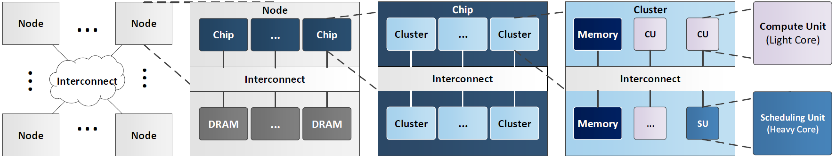
\includegraphics[width=1\textwidth]{Fig/figure3.png}
\end{figure}
%\textcolor{red}{Figure 3}

\subsection{Delaware Adaptive Run-Time System (DARTS)}
Since our main work is to apply Codelet model to brain-inspired computing, instead of implementing Codelet model, we borrowed DARTS - an implementation of Codelet model developed by the University of Delaware [4]. At present, a research team has already deployed it on Sunway supercomputer, the fastest supercomputer across the world, and conduct a serial of related research [5]. 
DARTS implements the Codelet AMM on real computer architectures for single-node shared memory multi-core computers from software level. With the help of DARTS, any existing computers can execute Codelet model under the node level. DARTS also allows users to set specific parameters of the abstract model, such as the number of clusters within a node, the number of CUs within a cluster, which allows us to conduct a more comprehensive analysis of the program performance. Moreover, DARTS has developed a complete runtime for Codelet model, including the implementation of Codelet and TP, the signal transmission among Codelets, and the different scheduling strategies of Codelet and TP.
DARTS is written in C ++ and uses a modular design that is highly portable and scalable. This is convenient not only to directly use the module, but also to improve the related modules for the brain-inspired computing features. (DARTS is an open source project, source code can be found here  \href{http://www.capsl.udel.edu/codelets/downloads/darts_20150318.tar.gz}{DARTS Source Code})
